\chapter{Podsumowanie}

Celem pracy było opracowanie oprogramowania przeznaczonego dla robota modularnego. W~pierwszym kroku dokonano analizy literatury, dzięki czemu wyłoniono najważniejsze cechy i~wymagania względem urządzenia. Dobór elementów elektronicznych powinien gwarantować pewien stopień autonomii każdego z segmentów -- umożliwić robotowi ruch oraz zapewnić jego zdolność do~wyznaczania swojej pozycji. Należało również znaleźć sposób na skomunikowanie modułów ze sobą oraz światem zewnętrznym. Ogólnym założeniem jest fakt, że oprogramowanie tak samo jak sam robot powinno być jak najbardziej uniwersalne. Ostatnim wnioskiem wyciągniętym na temat już istniejących konstrukcji jest potrzeba wprowadzenia narzędzi umożliwiających diagnostykę -- ze~względu na rozproszenie informacji w układzie konieczne jest archiwizowanie jego stanów, tak by~dało je się później odtworzyć. 

\begin{figure}[ht!]
    \centering
    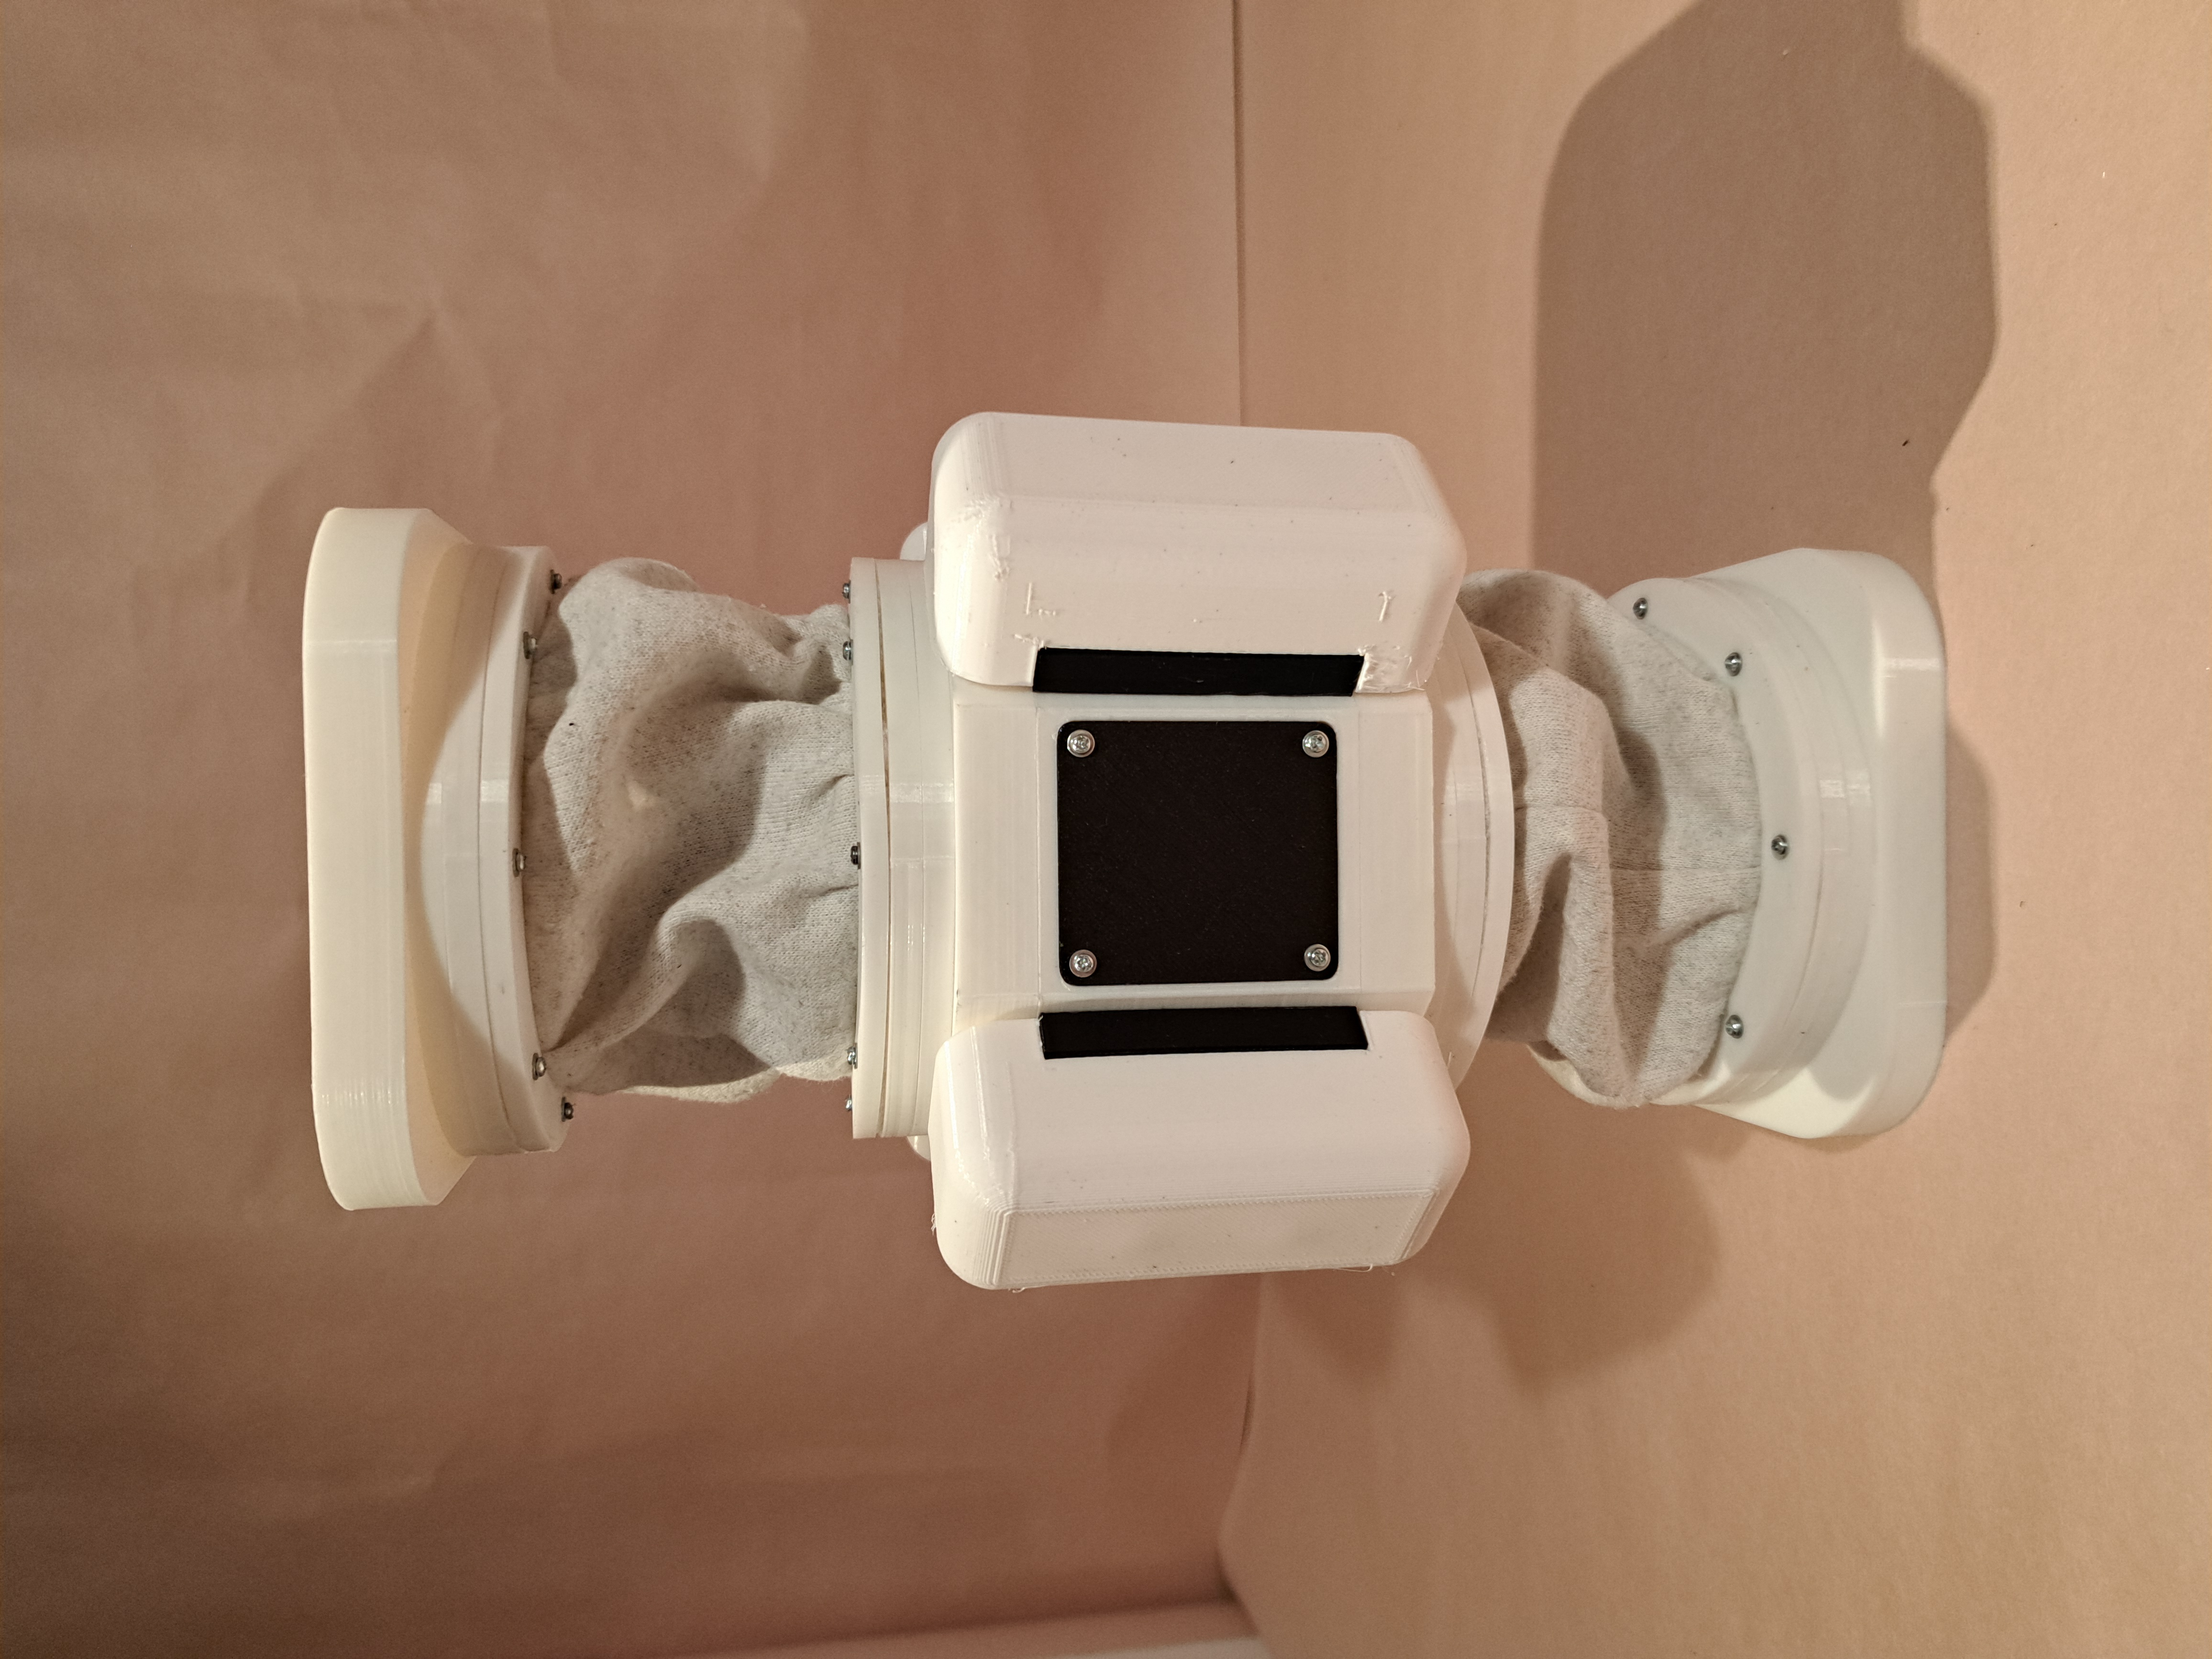
\includegraphics[width=0.8\linewidth, angle = -90 ]{rysunki/gizmo/gizmo_real.jpg}
    \caption{Fizyczny model robota}
    \label{fig: gizmo_real}
\end{figure} 

Przeanalizowano już gotową konstrukcję robota Gizmo i dobrano pod nią komponenty elektroniczne -- serwomechanizmy ST3020, akcelerometry ADXL345, nadajniki-odbiorniki MCP2551, wyświetlacz LCD oraz kartę microSD. Elementy pozwalają na: sterowanie robotem, ustalenie kątów obrotu każdego z serwomechanizmów, bieżący odczyt parametrów pracy a także prowadzenie kompleksowego dziennika aktywności. Na podstawie porównania rodzin Arduino, ESP32 oraz STM32 dokonano doboru płytki deweloperskiej stanowiącej serce układu. Mikrokontroler Nucleo-446RE spełnia wymagania odnośnie ilości pinów, pamięci ROM oraz RAM, a także potrzebnych interfejsów komunikacyjnych.

Zdecydowano się na zaimplementowanie dwóch magistrali komunikacyjnych. Pierwsza z nich oparta na protokole UART służyła do wymiany danych między panelem sterowniczym a modułem nadrzędnym, co pozwoliło na wygodne zarządzanie pracą urządzenia oraz monitorowanie jego statusu. Druga magistrala była wykorzystywana jedynie do wewnętrznej komunikacji między modułami i~została oparta na protokole CAN. Decyzja o tej metodzie komunikacji była oparta o trzy główne czynniki: wymaganie jedynie dwóch przewodów do zrealizowania połączenia, odporność na zakłócenia elektromagnetyczne, możlwość nadawania wiadomości przez każde urządzenia w sieci. 

Oprogramowanie zostało napisane w języku C z użyciem \textit{STM32CubeIDE}. Zastosowano wersjonowanie dzięki narzędziu \textit{git}. Całość kodu znajduje się na publicznym repozytorium oraz jest udostępniona na licencji open-source (GPLv3).

Ze względu na niejawność oprogramowania robotów wspomnianych we wstepie, cięzko jest porównać metodykę pisania kodu. Widoczne jest, że zastosowanie dwóch magistral -- wewnętrznej i zewnętrznej -- nie jest nowym podejściem i wydaje się być dobrą drogą. Sam dobór elementów elektronicznych, w tym mikrokontrolera, został dokonany kierując się podobnymi motywacjami -- dostosowując peryferia do warunków pracy robota. Elementem wspólnym jest również używanie akcelerometrów oraz enkoderów do wyznaczania pozycji urządzenia. Największą różnicą jest brak komunikacji bezprzewodowej, jedank jak wspomniano wcześniej jest ona możliwa do dodania w~kolejnych iteracjach projektu. 

Poprawność zaimplementowanych metod komunikacji zweryfikowano z użyciem aplikacji panelu sterowniczego. Natomiast jakość wysterowania serwomechanizmu oraz pomiarów jego kąta wyznaczono drogą eksperymentalną. Testy potwierdzają poprawność kodu, zatem wszystkie założenia pracy zostały zrealizowane zgodnie z oczekiwaniami. Oprogramowanie mogłoby być, rozszerzone o~szereg funkcjonalności, np.: związanych z wykrywaniem kolizji czy optymalizacji zużycia energii przez mikrokontroler oraz jego peryferia. Najbardziej korzystną zmianą, która powinna być wprowadzona w kolejnych wersjach to wykorzystanie testów jednostkowych (ang. \textit{Test Driven Development}) -- znacznie poprawiłoby to jakość oraz niezawodność kodu.

\section{Przyszłość projektu}
W ramach kolejnych etapów projektu należałoby stworzyć dedykowaną płytkę PCB oraz przeprowadzić testy oprogramowania przy prawdziwej pracy robota składającego się z kilku modułów.

Dodatkowo należałoby rozpocząć pracę nad bardziej złożonym algorytmem sterowania robota, w połączeniu z interfejsem umożliwiającym zadawanie konkretnych pozycji układu narzędziowego robota.
